% Tesis ITAM CLASS -- version 0.1 (13 - Abr - 2015)
% Clase para las tesis del ITAM
% 
% 13 - Abr - 2015 	Victor Martinez 	victor.martinez (at) itam.mx
% LICENSE: Creative Commons SA-BY 3.0
%
%
% Este documento presenta un ejemplo de uso de la plantilla
% El estudiante es libre de modificar este archivo a su gusto
% 
\documentclass{tesisITAM}
\usepackage[utf8]{inputenc}

\title{Predicción del Precio de una acción a partir de técnicas de Aprendizaje de Máquina}

\author{\textbf{DANAE SÁNCHEZ VILLEGAS}}
\degree{\textbf{INGENIERO EN COMPUTACIÓN}}
\advisor{DR. CARLOS FERNANDO ESPONDA DARLINGTON}
\year{2016}

\begin{document}

	\pagenumbering{gobble}
	\maketitle
	\publicationrights

	%%%%%%%%%%%%%%%%%%%%%%%%%%%%%%%%%%%%%%%%%%%%%%
	% ABSTRACT
	%%%%%%%%%%%%%%%%%%%%%%%%%%%%%%%%%%%%%%%%%%%%%%

	\begin{abstract}{spanish}
		Este documento presenta una plantilla para usar en las tesis y tesinas del ITAM. Se provee de manera gratuita y sin ninguna responsabilidad bajo la licencia \emph{creative commons BY-SA 3.0}.
	\end{abstract}

	\begin{abstract}{english}
		In this work we present a template for thesis and titulation works presented at ITAM. It is provided freely and without any responsability under the \emph{creative commons BY-SA 3.0}. 
	\end{abstract}


	\selectlanguage{english} 
	\setcounter{page}{1}
	\pagenumbering{roman}

	\tableofcontents
	\listoffigures
	\listoftables
	\newpage

	\pagenumbering{arabic}
	\setcounter{page}{1}

	%%%%%%%%%%%%%%%%%%%%%%%%%%%%%%%%%%%%%%%%%%%%%%
	% CONTENT
	%%%%%%%%%%%%%%%%%%%%%%%%%%%%%%%%%%%%%%%%%%%%%%
	 \chapter{Introduction}
\label{ch:introsm}
\begin{chapterquote}{Richard Feynman}
"Nature uses only the longest threads to weave her patterns, so
that each small piece of her fabric reveals the organization of
the entire tapestry."
\end{chapterquote}
Forecasting is of great interest in different areas of scientific, industrial, and commercial activities. It involves working with time series in a lot of cases. Time series are a collection of observations made sequentially through time \cite{chatfield2000time}. For example, the temperature in a specific region, the sales of a product in a store, and the electricity consumption in a fixed time interval.

Forecasting stock prices has been regarded as one of the most challenging applications of modern time series forecasting \cite{pai2005hybrid}. It involves a lot of uncertainties since its nature is essentially dynamic, non-linear, complicated, nonparametric, and chaotic. More important, financial forecasting is of great interest for investors since it helps to decide to invest in a stock or not as well as to sell it or not in order to get profits and avoid losing money.

The first attempt to describe a formula which expresses the likelihood of a market fluctuation was made by Louis Bachelier around one century ago. He was a young French mathematician convinced that the financial markets were a rich source of data for mathematicians and students of probability. 

Two other statisticians paid attention to stock market forecasting on the early 1900's. On 1934,  Holbrook Working found that although price levels do not follow a random pattern, price changes tend to be “largely random” \cite{bernstein1993capital}. Nineteen years later Kendall, confirmed Working's finding at his paper “The Analysis of Economic Time Series”. He declared that “the pattern of events in the price series was much less systematic than is generally believed” \cite{bernstein1993capital}. 

Although it may seem impossible to predict stock prices because of its seemingly random behavior, technical analysts believe that most information about the stocks is reflected in recent prices. Therefore, if trends in the movements are observed, then prices can be easily predicted \cite{patel2015predicting}. There are two types of analysis which usually investors perform before investing in a stock: fundamental analysis and technical analysis.

The fundamental analysis looks at intrinsic value of stocks, performance of the industry and economy, political climate etc. On the other hand, technical analysis is the evaluation of stocks by means of studying statistics generated by market activity. For example, past prices and volumes. Technical analysts use stock charts to identify patterns and trends that may suggest how a stock will behave in the future\cite{patel2015predicting}. This work focuses on this second type of analysis.

Stock market price forecasting models should be quick, adaptive, robust, and intuitive. A model that fits in all of these characteristics is the recurrent neural network. A recurrent neural network (RNN) is a neural network model proposed in the 80's for modeling time series \cite{pascanu2013difficulty}. Unlike standard artificial neural networks (ANN), it allows connections among hidden units associated with a time delay. Therefore, it can retain information about the past inputs. This characteristic makes the RNN model a great candidate for time series forecasting, and specifically, for stock market price forecasting.

Furthermore, RNN is a non- parametric model that, once trained, calculates the output very quickly. Parametric models assume forms of preset functions characterized by a number of parameters obtained from the sample. Conversely, non-parametric models have few assumptions about the form of the function.  

Traditional time series models like autoregressive moving average are parametric since they assume stationarity. Stationarity is a stochastic process where its parameters such as mean and variance do not change over time. Unfortunately, these barely happens in stock market prices. 

On the other hand, ANN is a very powerful machine learning model. However, it relies on the assumption of independence among the training and test examples \cite{lipton2015critical}. The state of the network is lost after processing each example. Commonly this is not a problem since each example is generated independently. But if a time or space relation exists between the examples as in this case, this is unacceptable.

RNNs do not make the stationary assumption and do not assume independence among the training and test examples. As stated before, they retain information about past inputs. This is why RNNs are widely used for time series applications, handwriting recognition \cite{graves2009offline}, speech recognition \cite{graves2013generating}, scene labeling \cite{pinheiro2014recurrent}, and forecasting stock markets \cite{hsieh2011forecasting}. 

\section{Objectives}
To design and implement a time series model for stock market price prediction using a recurrent neural network.

To compare the performance of the recurrent neural network model with two other predictive machine learning models, specifically, a feed forward artificial neural network model and a support vector machine model.

\section{Related Work}

A lot of research has been done around financial forecasting. Studies can be divided in two types of predictive models: traditional statistical models and machine learning models.

The first type includes the moving average, exponential smoothing, and the  autoregressive integrated moving average (ARIMA) models. These kind of models are linear in their predictions of the future values. They analyze historic data and attempt to approximate future values of a time series as a linear combination of these historic data \cite{shah2014performance}. 

On the other hand, artificial Neural Networks (ANN) and Support Vector Regression (SVR) are two machine learning algorithms widely used for predicting stock price values \cite{patel2015predicting}. Machine Learning uses a set of samples to generate an approximation of the underlying function that generated the data \cite{shah2014performance}.

In \cite{shah2014performance} they compared the performance of multilayer feed-forward neural network and the Elman neural network as representative of recurrent neural network for stock prediction. They found the neural network  better than Elman recurrent network and suggested to only use Elman model for historical data and research purposes. On the other hand, in \cite{kim2003financial} a support vector machine model was applied to predict the stock price index. Their experimental results showed that SVM provides a promising alternative to stock market prediction as it outperformed back-propagation neural network .

Researchers have also tried hybrid models, meaning a combination of two or more models that can be machine learning and/or traditional statistical models. In \cite{pai2005hybrid} a hybrid model of autoregressive integrated moving average (ARIMA) and a support vector machine model is presented to solve the stock price forecasting problem. They found that a simple combination of the individual models does not necessarily produce the best results and demonstrated great interest in the selection of optimal parameters for the model.

Another hybrid model is presented in \cite{rather2015recurrent}. Its model was constituted of two linear models,  ARIMA and exponential smoothing model and a non-linear model, recurrent neural network. Their results confirm the accuracy of the prediction performance of recurrent neural network compared to linear models.

This work compares the performance of three machine learning models: artificial neural network (ANN), support vector machine (SVM), and a deep learning model: recurrent neural network (RNN) with long short term memory networks (LSTM). ANN and SVM have been widely used for stock market forecasting and RNN with LSTM is a good option for problems where data is non-linear  as in this case, and where the patterns are difficult to be captured by traditional models.

\section{Scope}
In this study a novel stock market price prediction model is presented. This approach does not seek to get a number of next predictions but just the next one. Meaning, it requires a number $n$ of real past predictions and determines the $n+1$ price in the sequence. 

Another limitation is that just machine learning models were taken into account. Traditional models such as ARIMA are not compared. Finally, stock market’s movements are affected by many macro-economical factors such as political events, general economic conditions, bank exchange rates, investors’ expectations, and so on. The data used for training these models just incorporates the prices of a fixed time interval.

The rest of this work is organized as follows. In the next chapter machine learning and deep learning are introduced. First, we explain the McCulloch and Pitts's Neuron model in order to easily understand the traditional neural networks. Then, we explain support vector machine as an optimization of neural networks.

Next, we move to deep learning and study the recurrent neural networks as well as some techniques to optimize them. This includes regularization, gradient descent variants and gradient descent optimization algorithms.  

In  chapter 3, we explore the data and show how we can represent stock market prices as time series vectors. Then, we select the right parameters for each model and explain the criteria and metrics used to compare the models. Chapter 4 exhibits and analyzes  the results of the experiments and, finally, we draw the conclusions and propose future work at the final chapter.


	\chapter{Theoretical Framework}
\label{ch:theosm}

\begin{chapterquote}{Marquis of Halifax}
 "The best qualification of a prophet is to have a good memory. "
 \end{chapterquote}


\section{Machine Learning}
The process of learning has long fascinated people from many different disciplines such as psychology, biology, computer science, statistics, mathematics, and physics. 
Machine learning is about making computers modify or adapt their actions so that these actions get more accurate. Accuracy is measured by how well the chosen actions reflect the correct ones. As there are several ways to achieve this task there are different types of machine learning explained as follows \cite{marsland2015machine}:

\begin{itemize}
\item \textbf{Supervised Learning} a training set of examples with the correct responses or targets are provided and, based on this training set, the algorithm generalizes to respond correctly to all possible inputs.

\item \textbf{Unsupervised Learning} The algorithm tries to identify similarities between the inputs so that the inputs that have something in common are categorized together. In this type of learning correct responses are not provided.

\item \textbf{Reinforcement Learning} The algorithm gets told when the answer is wrong but does not get told how to correct it. Instead, it has to explore and try out different possibilities until it works out how to get the right answer. 

\item \textbf{Evolutionary learning} In this type of learning, biological evolution is seen as a learning process where the organisms adapt to improve their survival rates and chance of having offspring in their environment. It uses an idea of fitness which corresponds to a score for how good the solution is. 
\end{itemize}

\section{McCulloch and Pitts Neurons}
McCulloch and Pitts modeled an artificial neuron as a mathematical model in order to extract only the essentials required to accurately represent the entity, removing all the obscured details. They took into account three basic elements: a set of weighted inputs ($w_i$), an adder that sums the input signals, and an activation function that decides if the neuron fires to the current inputs.
\begin{figure}[h]
\centering
 
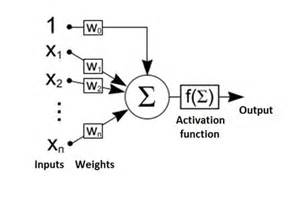
\includegraphics[width=10cm,height=5cm]{model_of_neuron.jpg}
\caption{McCulloch and Pitt's Neuron Model}
\label{fig:neuron}
\begin{minipage}{12cm}
    \footnotesize
    \center
    \emph \\ Taken from \cite{marsland2015machine}\\
    \end{minipage}
\end{figure}

The signals are added and if the sum is greater than a threshold $\theta$, it is activated. The mathematical expression is as follows:\\
\begin{equation} \label{eq:neuron}
h=\sum_{i=1}^{m} w_i * x_i + b
\end{equation}\ref{eq:neuron}

Thus, the output of the neuron is the sum of the $m$ inputs ($x_i$) multiplied by the weights ($w_i$). Furthermore, units can be given biases by introducing an extra input to each unit which always has a value of 1. The weight on this extra input is called the bias (b) and is equivalent to a threshold of the opposite sign \cite{polk2002cognitive}. 


\section{Artificial Neural Network}

A simple neural network is shown in Figure \ref{fig:nn}. It is formed by input units at the bottom, any number of intermediate or hidden layers, and a layer of output units at the top. Each of the units are  defined as a McCulloch and Pitts neuron. It should be noticed that connections within a layer from a higher to lower layer are forbidden. 

Since everything but the weights is known, learning or training refers to finding a set of weights so that for each input vector, the output vector produced by the network is sufficiently close to the desired output vector \cite{polk2002cognitive}. Thus, learning is translated to an optimization problem.

Gradient descent is an optimization algorithm used to find the parameters  that minimize a cost function. The derivative of the cost function with respect to the parameters is calculated and then equals zero. To calculate the derivative we can use backpropagation that can be seen as the recursive application of the chain rule.
%If the function is differentiable with respect to its parameters as in this case, gradient descent is a relatively efficient optimization method. This is because the computation of first-order partial derivatives with respect to all parameters is of the same computational complexity as just evaluating the function \cite{kingma2014adam}. 

In this case, the derivative with respect to the parameters turns out to be the error defined as the difference between the actual and the desired output vectors for every case. Now the problem is that there is not a direct solution for the partial derivatives with respect to the weights equals zero. Therefore, we cannot use the gradient descent for this last task but we can use a variant: stochastic gradient descent (SGD).
%escribir bien lo de igualar a cero
SGD updates the weights to the direction of the gradient. The error E in equation \ref{eq:error} is multiplied by a parameter called the learning rate $\nu$ and by the input $x_i$. This value is added to the weight ($w_{ij}$) for each j neuron and input i.

\begin{equation}
\label{eq:error}
E=(t_j - y_i)
\end{equation}

\begin{equation}
\label{eq:weight}
w_{ij} \leftarrow w_{ij}+\nu E * x_i
\end{equation} 
\centerline{where $0>=\nu<=1$ \\}

\begin{figure}
\center
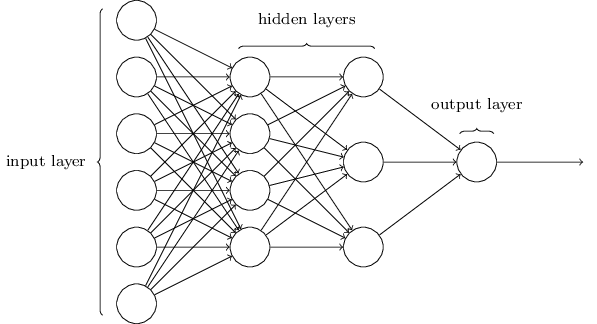
\includegraphics[width=10cm,height=5cm]{NN.jpg}
\caption{Neural Network}
\label{fig:nn}
\begin{minipage}{12cm}
    \footnotesize
    \center
    \emph \\ http://neuralnetworksanddeeplearning.com/chap1.html, by Michael Nielsen
    \end{minipage}
\end{figure}

Since the function is concave in W, the network is expected to get better answers until eventually its performance stops improving.

How much the weights are changed is controlled by the learning rate $\nu$. If it is too big, the weights will change a lot  making the network unstable so that it never settles down. On the other hand, if $\nu$ is too short it will be stable and resistant to errors and inaccuracies in the data, but it will take too long to learn. 

%The typical learning rate is between 0.1 and 0.4 \cite{marsland2015machine}.

\section{Support Vector Machine}
Support vector machine (SVM) can be seen as an optimization of a neural network. It uses the maximum margin hyperplane which gives the maximum separation between the decision classes. Meaning, SVM uses a linear model to implement nonlinear class boundaries mapping the input vectors x into a high-dimensional feature space. Then, a linear model constructed in the new space can represent a nonlinear decision boundary in the original space. Finally, in the new space, an optimal separating hyperplane is constructed \cite{kim2003financial}. 

The training examples that are closest to the maximum margin hyperplane are called support vectors and are the only ones used to define the binary class boundaries. Unlike neural networks, the only two parameters to tune are the kernel and the upper bound C for the non-separable cases in linear SVM \cite{drucker1999support}. Also, overfitting is unlikely to occur since it is usually caused by too much flexibility in the decision boundary and, in this case, the maximum hyperplane is relatively stable and gives little flexibility \cite{zhang1998forecasting}

The classifying rule is as follows:

\centerline{$\overleftarrow{w} * \overleftarrow{x_i} > 0  \rightarrow  positive $ \\}
\centerline{$\overleftarrow{w} * \overleftarrow{x_i} < 0  \rightarrow  negative $\\} 

The borders are calculated considering: \\
\centerline{ $\overleftarrow{y_i} (\overleftarrow{w}*\overleftarrow{x_i}+b)-1>=0$ \\}
where $y$ identifies the class $[1,-1]$\\

Therefore, the support vectors are defined as follows: \\
\centerline{$\overleftarrow{y_i} (\overleftarrow{w}*\overleftarrow{x_i}+b)-1=0$\\}

To maximize the distance between the borders of the classes for linearly separable classes we need to solve the next problem:

\centerline{$min \frac{1}{2}||\overleftarrow{w}||^2$\\}
\centerline{subject to $\overleftarrow{y_i} (\overleftarrow{w}*\overleftarrow{x_i}+b)-1>=0$ \\}

In case the classes are non linear, a looseness variable $C$ should be added: \\
\centerline{$min \frac{1}{2}||\overleftarrow{w}||^2+C\sum_{i}\xi_i$\\}
\centerline{subject to $\overleftarrow{y_i} (\overleftarrow{w}*\overleftarrow{x_i}+b)-1+\xi_i>=0$\\}
\centerline{$\xi_i>=0$}

Finally, the kernel is a function that transforms the data to a higher dimension. It substitutes the dot product between two vectors to build an extension of the observations. There are a few kinds of kernels. The main ones are the polynomial kernel(eq. \ref{eq:polyKernel}) and the gaussian (eq. \ref{eq:gaussKernel}) kernel.
\begin{equation} \label{eq:polyKernel}
K(X,X')=(X.X'+c)^{degree}
\end{equation}

\begin{equation} \label{eq:gaussKernel}
K(X,X')=e^{(-\gamma ||X-X'||^2)}
\end{equation}

%basar en apuntes de minería y buscar documentación
\section{Deep Learning}
As explained before, learning in the context of artificial neural networks refers to finding the adequate weights that make the network exhibit the desired behavior. Depending on the problem and how the neurons are connected, such behavior may require long causal chains of computational stages. Each stage transforms the aggregate activation of the network.

Deep Learning is about accurately assigning credit across many such stages \cite{schmidhuber2015deep}. This work will focus on recurrent neural networks, a subfield of deep learning in artificial neural networks (NNs).
%Another way of understanding deep learning is by studying neural networks as a representation learning method. This kind of methods allow a machine to be fed with raw data and to automatically discover the representations needed for detection or classification. Hence, deep learning methods are representation learning methods with multiple levels of representation. With the composition of enough transformations, very complex functions can be learned \cite{lecun2015deep}. 

\subsection{Recurrent Neural Networks}

A deep recurrent neural network (RNN) is a deep artificial neural network but with a different structure. In the deep case, connections among hidden units are allowed. Furthermore, these connections are associated with a time delay enabling the model to retain information about the past inputs. In this way, temporal correlations between events that are possibly far away from each other in the data can be discovered \cite{pascanu2013difficulty}.

\begin{figure}
\center
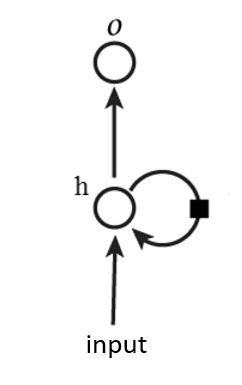
\includegraphics[width=3.5cm,height=5cm]{rnn.png}
\caption{Recurrent Neural Network}
\label{fig:r_nn}
\begin{minipage}{12cm}
    \footnotesize
    \center
    \emph \\ Taken from \cite{lecun2015deep}
    \end{minipage}
\end{figure}
For tasks that involve sequential inputs it results good to use RNNs. This is mainly because RNNs process an input sequence one element at a time and maintain in their hidden units a "state vector". This vector implicitly contains information about the history of all the past elements of the sequence.\cite{lecun2015deep} 

Sequential data arises through measurement of time series such as the rainfall measurements on successive days at a particular location, the daily values of a currency exchange rate and, to our interest, the stock market price in a time interval. The order of the prices as well as the relationships between them matter. Thus, to predict which is the most likely price to follow the sequence, it is important to retain this information.

% In this case the input data is the set of elements of a sentence or a set of sentences and the desired behaviour is to generate a new sequence that can adequately continue after the original one. Therefore, the target data for each element is the following one. 
The recurrent neural network receives an input vector $x=[x_1,...,x_T]$ which is passed through weighted connections to N recurrently connected hidden vector sequences $h^n=[h_1^n,...,h_T^n]$ and finally to the output vector sequence $y=[y_1,...,y_T]$ which will be compared to the target value for each observation. To compute the hidden layer activation the following equations are iterated from t=1 to T and from n=2 to N. \cite{graves2013generating}:

\begin{equation} \label{eq:hidden1}
h_t^1= H( W_{ih^1} * x_t + W_{h^1 h^1}*h^1_{t-1} + b^1_h)
\end{equation}

\begin{equation} \label{eq:hidden}
h_t^n= H(W_{ih^n} * x_t + W_{h^{n-1}  h^n} * h^{n-1}_t +W_{h^n h^n} * h^n_{t-1}+ b^n_h)
\end{equation}

The W terms denote the weight matrices that connect the input layer to the first hidden layer, two hidden layers between them or a hidden layer to an output layer. $H$ is the hidden layer function which usually is an application of a sigmoid function like the hyperbolic tangent. Finally, given the hidden sequences, the output sequence is computed as follows:

\begin{equation} \label{eq:output}
y_t=Y(\sum_{n=1}^{N} W_{h^{n}y} * h^n_t + b_y)
\end{equation}

Where $Y$ is the output layer function whose output vectors will need to be compared to the target values so that the network achieves the desired behaviour by minimizing the difference between both values.
%In Equation \ref{eq:error} the error was defined as this difference. Nevertheless, this definition is not adequate
The network now can be trained using the gradient descent to learn how the parameters, meaning the $W$ vector, should change to decrease the loss  $L(x)$. Therefore, the partial derivatives of the loss with respect to the weights should be computed. This can be achieved using backpropagation through time (BTT). The process computes the gradients of expressions through recursive application of the chain rule.

\subsubsection{Backpropagation Through Time}
BTT applied to RNNs have the constraint of sharing the parameters within each layer. As showed in  \ref{fig:unfold}, RNNs once unfolded in time can be seen as very deep feedforward networks in which all the layers share the same weights \cite{lecun2015deep}. Here, the model is presented as a deep multi-layer where each time step in the interval $[t,T]$ is a layer with N units each \cite{pascanu2013difficulty}. 

The constraint can be satisfied by adding the gradients for W at each time step. It can also be seen as an advantage since the network requires a smaller number of parameters than a non-recurrent neural network.

\begin{figure}

\center
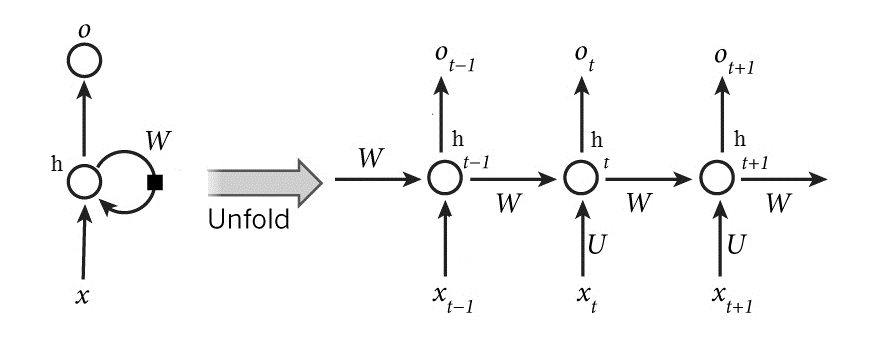
\includegraphics[width=10cm,height=5cm]{unfold.png}
\caption{Unfolded Recurrent Neural Network}
\label{fig:unfold}
\begin{minipage}{12cm}
    \footnotesize
    \center
    \emph \\ Taken from \cite{lecun2015deep}
    \end{minipage}
\end{figure}

%The key insight in BTT is that the calculation of the derivative of the objective with respect to the input of a module can be done by working backwards from the gradient with respect to the output of that module and repeating this process through all the layers or, in this case, through all the time steps \cite{schmidhuber2015deep}.

%a lo mejor aquí poner lo del -1

\subsubsection{RNNs Training Issues}
As described before, RNNs are very powerful dynamic systems. Unfortunately, training them has proved to be problematic. During the gradient backpropagation phase, the gradient signal can end up being multiplied a large number of times by the weight matrix associated with the connections between the neurons of the recurrent hidden layer. This causes that the backpropagated gradients either grow or shrink at each time step. Thus, the magnitude of weights in the transition matrix may have a strong impact on the learning process.

If the  weight matrix is smaller than 1, the gradient signal can get so small that so over many time steps it may vanish. Conversely, if the eigenvalue of the weight matrix is larger than 1, it can lead to a situation where the gradient signal is so large that it can explode causing learning to diverge. 

% The exploding gradients problem refers to the large increase in the norm of the gradient during training caused by the explosion of the long term components. On the other hand, the vanishing gradients problem is presented when long term components go exponentially fast to norm 0 making impossible for the model to learn correlation between temporally distant events \cite{pascanu2013difficulty} which was the main reason for choosing RNNs for this work. 

\subsubsection*{The exploding gradients problem}
 The fact that the norm of the gradient increases during training is a problem because the computation becomes inefficient and also increases the response time. One simple mechanism to deal with this problem is to rescale it whenever it goes over a threshold. To choose wisely the threshold, one good heuristic is to look at statistics on the average norm over a sufficiently large number of updates. In this way, we can handle very abrupt changes in norm as it adapts the learning rate based on the norm of the gradient  \cite{pascanu2013difficulty}.

\subsubsection*{The vanishing gradients problem}

The vanishing gradients problem makes it difficult to learn to store information. Having a longer memory has a establishing effect, because even if the network cannot make sense of its recent history, it can look further back in the past to formulate its predictions \cite{graves2013generating}.

%This amnesia makes them prone to instability when generating sequences. The main problem is that if the network's predictions  are only based on the last few inputs, and these inputs were themselves predicted by the network, it has little opportunity to recover from past mistakes.

A lot of research work has been made to propose solutions to this problem. The main idea is to augment the network with an explicit memory. The first proposal of this kind is the long short-term memory (LSTM) network used in this work. The LSTM has complicated dynamics that allow easily “memorizing” information for an extended number of time steps \cite{zaremba2014recurrent}.

\subsubsection{Long Short-Term Memory Networks}
Long Short-term Memory (LSTM) is an RNN architecture. The difference is that instead of using a sigmoid function as hidden layer function, LSTMs use memory cells to store information. The new architecture has three gates and a memory cell. The gates are for input, forget, and output functions. The memory cell has a connection to itself at the next time step with a weight of one, meaning it copies its own real-valued state and accumulates the external signal \cite{lecun2015deep}. Thus, it can decide to overwrite the memory cell, retrieve it, or keep it for the next time step\cite{zaremba2014recurrent}. 

LSTMs are better at storing and accessing information than standard RNNs. The cells improve the performance when finding and exploiting long range dependencies in the data. Additionally, the full gradient can be calculated with backpropagation through time as well.\cite{graves2013generating}

\begin{figure}
\center
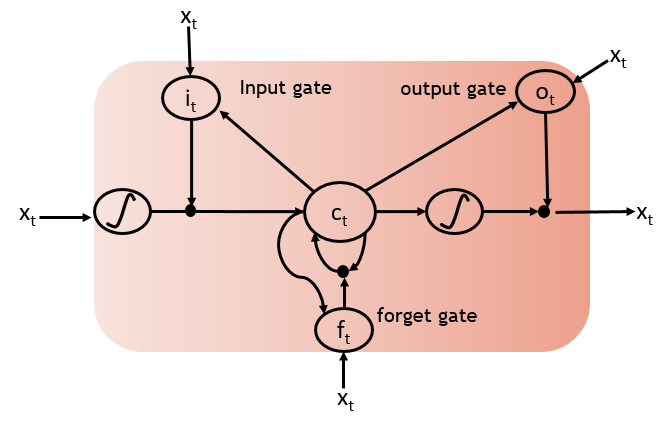
\includegraphics[width=10cm,height=5cm]{gates.PNG}
\caption{Long Short Term Memory Network}
\label{fig:lstm}
\begin{minipage}{12cm}
    \footnotesize
    \center
    \emph \\ Based on \cite{greff2016lstm}
    \end{minipage}
\end{figure}

The forget gate $f_t$ decides the content to keep for each time step $t$. It is a sigmoid function that takes into account the $h_{t-1}$ and the present input $x_t$ and returns a number between 0 and 1 where 0 means "forget it" and 1 means "keep it". 

The next step is to calculate the input gate to decide which values to update using a sigmoid function (Eq. \ref{eq:input}). Then, the new candidates are computed by a tanh function (Eq. \ref{eq:candidate}), and the memory cell update is done by combining the previous functions as explained in Eq. \ref{eq:update}.

\begin{equation} \label{eq:forget}
f_t=\sigma(W_f*(h_{t-1},x_t)+b_f)
\end{equation}
\begin{equation} \label{eq:input}
i_t=\sigma(W_i*(h_{t-1},x_t)+b_i)
\end{equation}
\begin{equation} \label{eq:candidate}
C'_t=tanh(W_C*(h_{t-1},x_t)+b_C)
\end{equation}
\begin{equation} \label{eq:update}
C_t=f_t*C_{t-1}+i_t*C'_t
\end{equation}

Finally, the output function decides which parts of the memory cell to return with another sigmoid function (Eq. \ref{eq:output}). Lastly the $h_t$ is calculated (Eq. \ref{eq:hidden}) with the output function and a tanh function of the memory cell to push the values into the interval [-1,1].

\begin{equation} \label{eq:output}
o_t=\sigma(W_o*(h_{t-1},x_t)+b_o)
\end{equation}
\begin{equation} \label{eq:hidden}
h_t=o_t*tanh(C_t)
\end{equation}

\subsection{Regularization}

Successful applications of neural networks require good regularization. Although deep neural networks with a huge number of parameters are very powerful machine learning systems, they tend to overfit at training time causing an error with great variance. 

Fortunately, dropout is a technique for addressing this problem. The key idea is to randomly drop units (along with their connections) from a neural network during training in order to prevent the units from co-adapting too much \cite{srivastava2013improving}. However, when working with recurrent neural networks and specifically with LSTM networks it is not desired to erase all the information from the units. It is extremely important that the units remember events that occurred many time steps in the past. This is the reason for \cite{zaremba2014recurrent} to only use drop out in the non-recurrent connections. 

Nevertheless, in \cite{gal2015theoretically} they develop a technique to effectively use drop out in all connections called Variational RNN. In this dropout variant, the same dropout mask at each time step is repeated for both inputs, outputs, and recurrent layers, so the same network units are dropped at each time step. 
%The interpretation for this work (character-level language modelling) is to force the model not to rely on single characters for its task.
%Finally, they found that the optimal dropout probabilities are between 0.3 and 0.5.

\subsection{Gradient Descent Variants}
As previously introduced, gradient descent is an optimization algorithm used to find the parameters that minimize an objective function. There are three variants of the gradient descent: batch gradient descent, stochastic gradient descent, and mini-batch gradient descent. The variants differ in how much data is used to compute the gradient of the objective function. 

The first variant computes the gradient of the cost function with respect to the parameters ($\theta$) for the entire dataset as in \ref{eq:batchgd}.

\begin{equation} \label{eq:batchgd}
\theta=\theta-\eta * \Delta_\theta * J(\theta)
\end{equation}

The second variant computes a parameter update for each training example $x_i$ and target $y_i$ \ref{eq:sgd}.
\begin{equation} \label{eq:sgd}
\theta=\theta-\eta * \Delta_\theta; * J(\theta;x_i;y_i)
\end{equation}

Where $\eta$ is the learning rate.

The problem with the batch gradient descent is that it can be very slow and it does not allow updating the model with new examples on-the-fly. The stochastic gradient descent solves this problem and is faster than the batch gradient descent, but it performs updates with high variance causing the objective function to fluctuate heavily.  

Finally, the mini-batch gradient descent performs an update for every mini-batch of $n$ training examples as in equation \ref{eq:mbgd} \begin{equation} \label{eq:mbgd}
\theta=\theta-\eta * \Delta_\theta * J(\theta;x_{i:i+n};y_{i:i+n})
\end{equation}

In this way, the mini-batch gradient descent reduces the variance of the updates, is faster than the first variant and allows the model to update with examples on-the- fly. Therefore, this third option is the chosen one for this work \cite{ruder2016overview}. 

\subsection{Gradient Descent Optimization Algorithms}
%To our knowledge, mini-batch Gradient Descent (SGD) is the best option to find the parameters that minimize an objective function. Mini-batch gradient descent is stochastic since the objective function is composed of a sum of subfunctions evaluated at different subsamples of data. Another source of noise may also come from dropout regularization \cite{kingma2014adam}. 
Choosing the proper learning rate $\eta$ is a difficult and important task. Using the same learning rate for all parameter updates may not be the best choice if the data is sparse and the features have different frequencies. In this case, it would be better to perform a larger update for rarely occuring features. Another challenge is to avoid getting trapped in a local minima when working with non-convex objective functions as is the usual case in deep learning. For these cases, efficient stochastic techniques as the ones explained in the following are required \cite{ruder2016overview}.
%fuente:http://sebastianruder.com/optimizing-gradient-descent/

The main algorithms used to avoid those challenges in deep learning applications are: Momentum, Nesterov and the accelerated gradient, Adagrad, RMSPop, and Adam. The first two algorithms adapt the updates to the slope of the error function and, thus, speed up SGD. The last ones adapt the updates to each individual parameter to perform larger updates for infrequent parameters and smaller updates for frequent parameters. This makes the algorithm well-suited for dealing with sparse data \cite{ruder2016overview}.

%Momentum \cite{qian1999momentum} is a method that helps accelerate gradient descent in the relevant direction and dampens oscillations by taking in account a fraction $\phi$ of the update vector of the past time step to the current update vector:

%\begin{equation}
%\theta=\theta-(\nu_t=\phi \nu_{t-1} + \eta \Delta_\theta J(\theta))
%\end{equation}
%Where $\phi$ is the momentum term usually set to 0.9.

%The momentum term increases for dimensions whose gradients point in the same directions and reduces updates for dimensions whose gradients change directions. As a result, we gain faster convergence and reduced oscillation.
%chance y quitar esto

%Nesterov accelerated gradient \cite{nesterov1983method} not only uses the momentum term $\phi \nu_{t-1}$  to move the parameters $\theta$; but it also computes $\theta - \phi \nu_{t-1}$ to give an approximation of the next position of the parameters.  
%\begin{equation}
%\theta=\theta-(\nu_t = \phi \nu_{t-1} + \eta \Delta_\theta J(\theta - \phi \nu_{t-1})
%\end{equation}
  
The name Adam comes from adaptive moment estimation. It combines the advantages of AdaGrad and RMSProp \cite{kingma2014adam}. As RMSprop, ADAM  stores an exponentially decaying average of past squared gradients $\nu_t$: %In addition, Adam keeps an exponentially decaying average of past gradients $m_t$ similar to momentum:
\begin{equation}
m_t=\beta_1 m_{t-1} + (1-\beta_1)g_t
\end{equation}

\begin{equation}
\nu_t=\beta_2 \nu_{t-1} + (1-\beta_2)g^2_t
\end{equation}

Where $m$ and $\nu$ are estimates of the first moment and the second moment of the gradients respectively, meaning the mean and the uncentered variance. Both are initialized as vectors of zeros and, thus, they are biased towards zero. Then, they are corrected as follows:
\begin{equation}
\hat{m_t}=\frac{m_t}{1-\beta^t_1}
\end{equation}

\begin{equation}
\hat{\nu_t}=\frac{\nu_t}{1-\beta^t_2}
\end{equation}

Finally, the next equation is computed to update the parameters:
\begin{equation}
\theta_{t+1}=\theta_t-\frac{\eta}{\sqrt[2]{\hat{\nu_t}} + \epsilon} \hat{m_t} 
\end{equation}

Where $\epsilon$ is a smoothing term to avoid the zero division. The default proposed values are $10^{-8}$ for $\epsilon$, 0.9 for $\beta_1$ and 0.999 for $\beta_2$.
%falta fuente

%Adam is better than Adagrad because it resolves the main disadvantage of it that is its accumulation of the squared gradients in the denominator that divides the learning rate\cite{duchi2011adaptive}. Since every added term is positive, the accumulated sum keeps growing during training causing the learning rate to shrink and eventually becomes infinitesimally small, so the algorithm cannot acquire additional knowledge\cite{ruder2016overview}. 

It has been empirically shown that Adam works well in practice and better than other adaptive-learning algorithms including the RMSProp and AdaGrad. Therefore it is the one chosen for this work.
%fuente!!!!!!!!!!!!!!!!!!!!!!!!!!!!!!!!!!!!!!!!!!!!!!!!!
-

    \chapter{Solution Design}
\label{ch:design}

\begin{chapterquote}{Ludwig Wittgenstein}
	The limits of my language mean the limits of my world.
\end{chapterquote}

\section{Problem Description}

Twitter is a microblog service where users write state messages called \textbf{tweets}. The length of these messages are lower or equal to 145 characters and they use to express people's opnions about several topics. The set of all these tweets generates a great amount of information that can be used by diffent kinds of users such as analysts, consultors, community managers, market researchers, etc..

The model was implemented in Keras, a high-level neural networks library written in Python. It can run on top of either TensorFlow or Theano. It can work with the CPU or with the GPU, supports recurrent networks, and arbitrary connectivity schemes including multi-input and multi-output training. 

\section{Text representation}

The first step is to decide the information representation. As explained before predicting one character at a time is more interesting from the perspective of sequence generation, because it allows the network to invent novel words and strings. Therefore, the model will be character-level. To represent the text of M different characters and length N, we focus on specific text windows of length F that we check every step size S. Then, the number of sequences is given by the integer division: $NbSq=(N-F)/S$. For example, if we have the phrase "The limits of my language are the limits of my world" we have a text of length $N=52$ and $M=19$ different characters. Then if we set $F=4$ and $S=2$ we have 24 sequences whose target is its next character as showed in table \ref{tab:seqch}.Training the RNN on many shorter sequences is just as effective than training the whole string at once, provided they are several hundred characters or more long. This is a better choice since as explained before, to compute the exact gradient of the log probability of the training set, the RNN needs to process the entire training set sequentially and store the hidden state sequence in order to apply BTT. This task is infeasible due to the size of the training sets as well as unnecessary\cite{sutskever2011generating}.

\begin{table}{}

\begin{tabular}{c c}
\textbf{Phrase: }&The limits of my language are the limits of my world \\
\end{tabular}
\begin{tabular}{c c c c c c c c c c c c c c c c c c c c c}
\textbf{No.}&0&1&2&3&4&5&6&7&8&9&10&11&12&13&14&15&16&17&18\\
\textbf{Characters:}& " "& T& a& d& e& f& g& h& i& l& m& n& o& r& s& t& u& w& y\\
\end{tabular}

\begin{tabular}{c c c c c c c c c c c c c c}
\textbf{Sequence:} &0&1&2 & 3 &4&5&6&7&8&9&10&11\\
\textbf{Chars:} &The &e li&limi&mits&ts o& of &f my&my l& lan&angu&guag&age\\ 
\textbf{Next character: }&l&m&t&" "&f&m&" "&a&g&a&e&a\\
\textbf{Sequence:} &12&13&14&15&16&17&18&19&20&21&22&23\\
\textbf{Chars:} &e ar&are &e th&the &e li&limi&mits&ts o& of &f my&my w& wor\\
\textbf{Next character: }&e&t&e&l&m&t&" "&f&m&" "&o&l\\
\end{tabular}

\caption{Sequences of Characters}
\label{tab:seqch}

\end{table}


Next we have to use the one-of-K representation for each character in each sequence. Since the number of text classes is the number of different characters for each sequence $(ns,f);  ns \in NbSq; f \in F $, we need a vector of size $M$ where every element is a zero except for the number of element that corresponds to the character. For example, if $ns=13$ and $f=1$ the character is 'a' and therefore its one-of-K representation is: $[0,0,1,0,0,0,0,0,0,0,0,0,0,0,0,0,0,0,0,]$. 
Now we have a matrix of dimensions: $SxFxM$ that represents the text of length N and that will be the input of the network. Conversely, the target next characters are mapped to a the one-of-K representation. This will model a $NbSq x M$ matrix. As in \cite{sutskever2011generating}, we used sequences of length $F=250$. 

\section{Network Architecture}

The model has an input, a hidden and an output layer. The input layer has the same number as the total of sequences $(NbSq)$, each of dimensions $FxM$. The network has one single hidden layer with 1000 LSTM units as suggested in \cite{graves2013generating}.The LSTM has a drop out of 0.5 implemented as suggested in \cite{gal2015theoretically} in both, recurrent and non-recurrent connections. Finally, because this is a classification problem we use a fully connected output layer with the same number of neurons as unique characters ($M$). It uses the softmax function as activation function to make predictions for each of the classes and the cross-entropy function as loss function. The ADAM SGD optimizer in order to adapt the learning rate dynamically as the data is sparse. The next character is then the one with the greatest probability that is computed at the last step. Figure \ref{fig:netarch}  Where $x_{i}$'s are the $M$ input sequences and $x_o$ is the predicted next character. Of course, it is needed to translate the prediction from one-of-K representation to character representation at the end of the process

\begin{figure}[h]
\centering
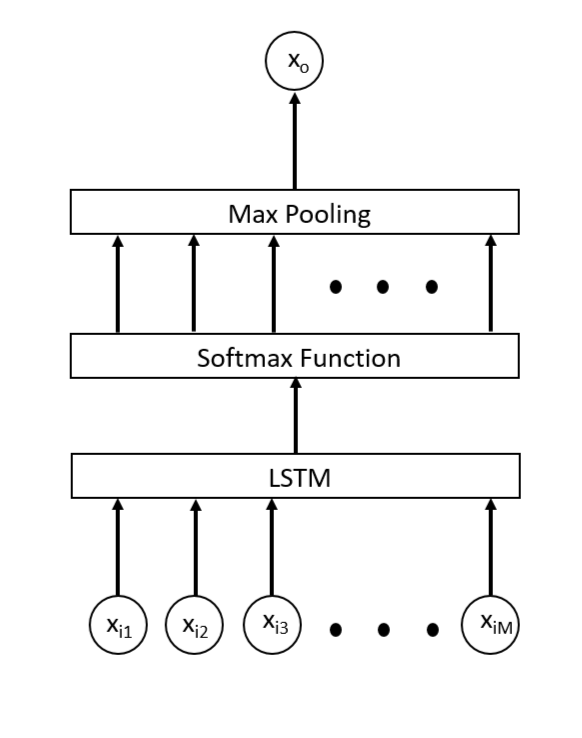
\includegraphics[width=6cm,height=6cm]{Modelo1.PNG}
\caption{Network Architecture}
\label{fig:netarch}
\end{figure}

























	% \include{Chapters/relatedwork}

	% \include{Chapters/method}

	% \include{Chapters/results}
 
	% \include{Chapters/conclusions}

	%%%%%%%%%%%%%%%%%%%%%%%%%%%%%%%%%%%%%%%%%%%%%%
	% APPENDIX
	%%%%%%%%%%%%%%%%%%%%%%%%%%%%%%%%%%%%%%%%%%%%%%
	\appendix
	% \include{Chapters/appendixA}

	%%%%%%%%%%%%%%%%%%%%%%%%%%%%%%%%%%%%%%%%%%%%%%
	% BIBLIOGRAPHY
	%%%%%%%%%%%%%%%%%%%%%%%%%%%%%%%%%%%%%%%%%%%%%%
	\clearpage
	\addcontentsline{toc}{chapter}{References} %Añadimos la bibliografia a la lista de contenidos.
	
	%%%%%%%%% Referencias usando el sistema embedido %%%%%%%%%%%
	% e.g. (Ejemplo tomado de https://en.wikibooks.org/wiki/LaTeX/Bibliography_Management)
	%
	% \begin{thebibliography}{9}
	%
	%	\bibitem{lamport94}
    %			Leslie Lamport,
    %			\emph{LaTeX: a document preparation system},
    %			Addison Wesley, Massachusetts,
  	%			2nd edition,
    % 			1994.
    %
	% \end{thebibliography}

	%%%%%%%%% Referencias usando bibtex %%%%%%%%%%%
	\bibliographystyle{plain}
	\bibliography{references} 

\end{document}